\index{Database!Log-in}
\index{Log-in!Database}
\begin{enumerate}
\item \gdprojects{} are stored in  a \gddb{}. Before you can access a \gdproject{}, you have to log in to the \gddb{}. 
\item The log-in dialog for the \gddb{} (\bxfigref{dblogin}) appears automatically the first time you need it (e.g. when you try to open or create a \gdproject{}). 

\begin{figure}[h]
\begin{center}
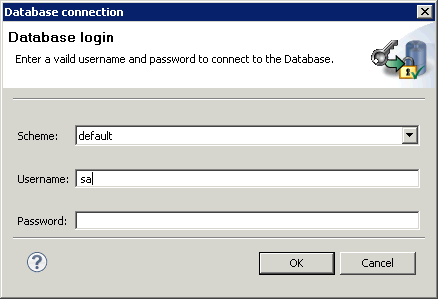
\includegraphics[width=0.5\textwidth]{Tasks/Database/PS/dblogin}
\caption{Database login}
\label{dblogin}
\end{center}
\end{figure}

\bxtipp{If you are using the default demo (embedded) \gddb{}, you will automatically be logged into the \gddb{}. }

\bxwarn{We do not recommend using the embedded \gddb{} for productive use of \app{}.} 

\item Select the \gddb{} you want to use and enter your username and password.

\bxtipp{If you previously had another \app{} version installed, you may see the information that your current \gddb{} version is not compatible with the latest version. If this is the case, then you can automatically migrate your \gddb{} \bxpref{DBMigrate}.}

\item If you want to save your \gddb{} password, select the checkbox to store it in the secure store. You can edit your password settings in the preferences via: \\
\bxname{General/Security/Secure Store}. 
\item Once you have opted to save your password, you can also choose whether you want to perform an automatic login to this \gddb{} when you use this workspace. If you select this option, then the next time you open \app{} and e.g. select:\\
\bxmenu{Test}{Open}{}\\
you will be automatically connected to this \gddb{} with the username and password you entered.
\item You can change your auto-login details or select another \gddb{} at any time by selecting:\\
\bxmenu{Test}{Select database...}{}
\end{enumerate}

